% ==========================================================
\section{Tooling Support for UVL-Based Feature Models}
\label{sec:sota_uvl_tools}
% ==========================================================

As the Universal Variability Language has established itself as a common exchange format for feature models across research and industry, a growing ecosystem of tools has emerged to support model authoring, visualization, and automated analysis.
The following subsections survey the most prominent solutions currently available, covering both dedicated language-server extensions for text-based editing and fully \gls{ide} that combine editing with graphical exploration and automated reasoning.

% ----------------------------------------------------------
\subsection{Universal Variability Language Server}
\label{subsec:uvls}
% ----------------------------------------------------------
 
The \gls{uvls} is a \gls{lsp} implementation specifically designed for \gls{uvl}, providing editing assistance for the manual authoring of large feature models.
Conforming to the \gls{lsp} protocol, \gls{uvls} integrates easily into any compatible editor.
Integrations for Visual Studio Code and NeoVim are already available~\cite{loth_uvls_2023, noauthor_universal-variability-languageuvl-lsp_2025}.

\gls{uvls} performs multi-level static analysis as the user types, providing immediate feedback without requiring explicit validation steps.
Syntactic validation leverages a tree-sitter-based parser~\cite{loth_uvls_2023} to detect grammar violations and pinpoint exact error locations.
For semantic analysis, \gls{uvls} integrates the SMT solver Z3~\cite{noauthor_z3proverz3_2026} to identify modeling anomalies such as void models, dead features, contradictions, and redundant tautologies~\cite{loth_uvls_2023}.
 
To further support model authoring, \gls{uvls} provides context-sensitive auto-completion suggesting valid group types, numerical attributes, and importable submodels based on UVL grammar.
Advanced syntax highlighting differentiates grouping keywords, feature identifiers, types, attributes, and constants, enhancing code readability.
Reference handling enables users to locate all usages of a feature or attribute across cross-tree constraints and perform synchronized renames.
 
For interactive product configuration, \gls{uvls} provides a dedicated editor supporting decisions across all UVL domains with real-time validity feedback.
Configuration choices can be rendered as inline code annotations within the source model, improving traceability.
Finally, \gls{uvls} can generate a Graphviz~\cite{noauthor_graphviz_nodate} \texttt{.dot} file from the feature model, which in environments such as VSCode is rendered and refreshed in real time as the user edits the source.

% ----------------------------------------------------------
\subsection{FeatureIDE}
\label{subsec:featureide}
% ----------------------------------------------------------
 
FeatureIDE is an open-source, Eclipse-based framework for \gls{fosd} that has become the de facto standard in both academic research and industrial practice.
It supports multiple composition paradigms and implementation languages, including FeatureHouse, FeatureC++, Java, C++, Haskell, and XML, making it adaptable to diverse development contexts~\cite{kastner_featureide_2009, noauthor_featureidefeatureide_2026}.
 
The framework supports the complete \gls{fosd} workflow end-to-end.
A graphical editor enables engineers to construct and maintain feature models, which are persisted in machine-readable formats suitable for automated analysis.
For configuration, a dedicated user interface allows users to select features for specific product variants, providing immediate validation of conflicting specifications.
Background composition assembles program artifacts automatically as feature selections or implementations change.
Compilation errors are propagated and annotated directly in the affected source files.
FeatureIDE's extensible architecture allows researchers to integrate custom format parsers, type-checkers, and refactoring tools.
The effort required for advanced components often varies because such components are not always generalizable across different implementation strategies~\cite{kastner_featureide_2009}.
 
\gls{uvl} is supported natively as an alternative textual format through a Clojure-based parser library and a thin integration layer that translates \gls{uvl} elements into FeatureIDE's internal model representation~\cite{sundermann_integration_2021}.
Parsing errors are reported with precise line and column information, including semantic validation such as constraint reference checking handled by FeatureIDE itself.
\gls{uvl}'s composition mechanism is fully leveraged: features from referenced submodels are visually distinguished by a sky-blue border and alias prefix.
They remain read-only in composed views while being editable in their source submodels.
However, \gls{uvl} cardinalities (e.g., \texttt{[3..6]}) are not yet supported, requiring tool-specific metadata to be stored as generic feature attributes as a workaround~\cite{sundermann_integration_2021}.

\begin{figure}[ht]
    \centering
    \begin{subfigure}[t]{0.49\textwidth}
        \centering
        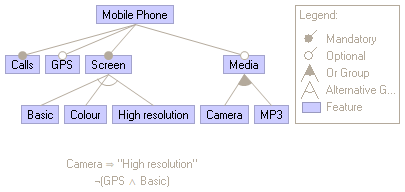
\includegraphics[width=\linewidth]{figures/featureide_mobile_phone.png}
        \caption{Rendered by FeatureIDE~\cite{noauthor_featureidefeatureide_2026}.}
        \label{fig:featureide_mobile_phone}
    \end{subfigure}
    \hfill
    \begin{subfigure}[t]{0.49\textwidth}
        \centering
        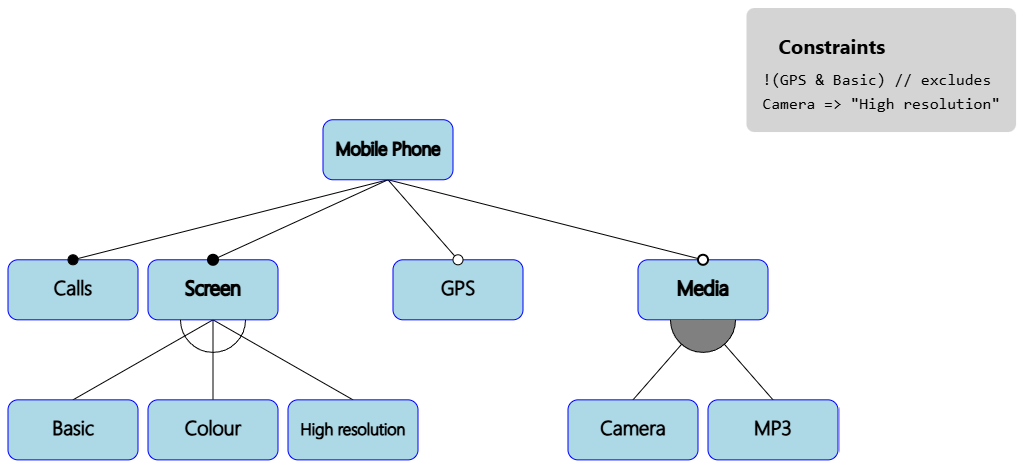
\includegraphics[width=\linewidth]{figures/flamapy_ide_mobile_phone.png}
        \caption{Rendered by \texttt{flamapy.ide}~\cite{noauthor_flamapyflamapy-ide_2026}.}
        \label{fig:flamapy_ide_mobile_phone}
    \end{subfigure}
    \caption[Graphical representation of mobile phone]{Different graphical representations of the mobile phone feature model.}
    \label{fig:representations_mobile_phone}
\end{figure}

% ----------------------------------------------------------
\subsection{flamapy.ide}
\label{subsec:flamapy_ide}
% ----------------------------------------------------------

\texttt{flamapy.ide}~\cite{benitez_uvl_2025, noauthor_flamapyflamapy-ide_2026} is a browser-based IDE built on the open-source \texttt{flamapy} framework~\cite{galindo_flama_2023, noauthor_flamapyflamapy_2026}.
Rather than requiring users to install native applications or Python environments, the tool adopts a fully client-side architecture by compiling \texttt{flamapy} to WebAssembly via Pyodide~\cite{noauthor_pyodidepyodide_2026}.
All computations execute directly in the user's browser.
There are no dependency-management overheads, and sensitive feature models remain client-side without transmission to remote servers.
 
The \gls{ide} embeds a Monaco-based code editor with full \gls{uvl} support~\cite{benitez_uvl_2025}.
As users type, the editor automatically parses the document, providing syntax highlighting and error detection so modeling mistakes surface immediately rather than deferring to an explicit validation step.
The user interface of \texttt{flamapy.ide} is illustrated in Figure~\ref{fig:flamapy_ide_ui}.

Additionally, feature models can be rendered as interactive tree graphs using D3.js~\cite{noauthor_d3d3_2026}, enabling intuitive navigation through the feature hierarchy.
This tight coupling between textual and graphical representations ensures that any valid edit to the \gls{uvl} source is immediately reflected in the diagram.

\begin{figure}[ht]
    \centering
    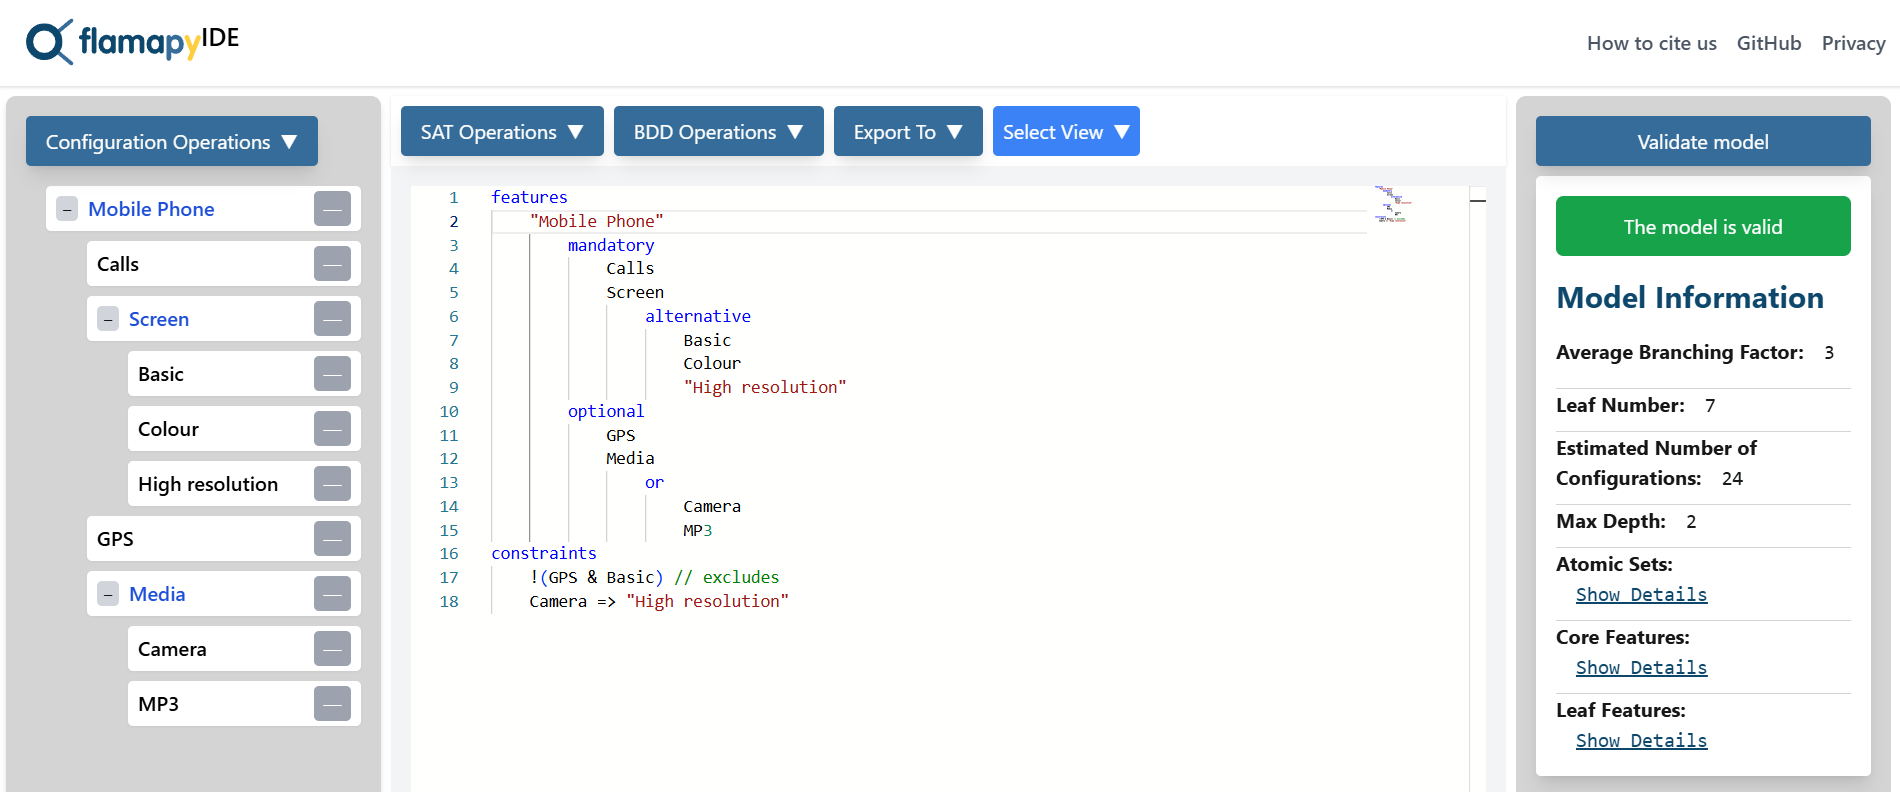
\includegraphics[width=\linewidth]{figures/flamapy_ide_ui.png}
    \caption[User Interface of \texttt{flamapy.ide}]{The \texttt{flamapy.ide} user interface with the \gls{uvl} code editor~\cite{noauthor_flamapyflamapy-ide_2026}.}
    \label{fig:flamapy_ide_ui}
\end{figure}

Beyond editing and visualization, \texttt{flamapy.ide} exposes automated reasoning through dedicated analysis backends.
SAT-based routines use propositional satisfiability solving to check model satisfiability and to count valid configurations.
BDD-based operations implement Binary Decision Diagrams for efficient reasoning over feature models.
These support configuration counting, core feature detection, and feature-inclusion probability estimation.
An interactive product configurator guides feature selection step by step and validates each choice against model constraints, providing real-time feedback on configuration validity~\cite{benitez_uvl_2025}.